%************************************************
\chapter{Materials}
\label{chp:Mat}
%************************************************


\section{Study Areas}\label{sec:StudyAreas}\index{study area}

The research studies, which are compiled in the present work, were conducted using remote sensing data and ground based measurements
from different test sites\index{test site|see{study area}} 
(see Figures~\ref{fig:TestSites_BY} and \ref{fig:TestSite_NVI}, and Table~\ref{tab:TestSites}).
The selection \graffito{Selection criteria for the study areas in \emph{Bavaria}.} of the test sites in \emph{Bavaria}, 
Germany, was made in order to best meet the following criteria:

\begin{itemize}
	\item Field inventory measurements of recent date are available for larger contiguous forested areas.
	\item Lapse of time between the acquisition of the airphotos and the ground based measurements is as short as possible.
	\item Test sites represent different forest conditions, including topography, climate, tree species, tree species mixture, 
		and forest management practice.
\end{itemize}

\noindent The test site on \emph{\ac{NVI}} was selected \graffito{A comparative analysis of \ac{ALS}- and \ac{DAP}-based height data
	was possible for the \ac{NVI} test site.}
in order to scrutinize the developed methods 
under largely different conditions, \ie, among other factors, the areal extent of the test site, the prevailing tree species, the applied forest management, 
and the different strategy for ground data acquisition. Timely coincident data of \ac{ALS} and aerial photography were available for the \ac{NVI} area,
which allowed for a comparative analysis of both remote sensing data types for use in forest inventory applications.   

\begin{threeparttable}[t]
	\myfloatalign
	\caption[Overview of test sites.]{Overview of the different test sites in Bavaria, Germany, and British Columbia, Canada.}
	\label{tab:TestSites}
	\small
	\begin{tabularx}{\textwidth}{p{2.7cm}p{.7cm}p{2.6cm}X}
		\toprule
		\tableheadline{Test site} & \spacedlowsmallcaps{Area} \linebreak \footnotesize{[km\textsuperscript{2}]} & \spacedlowsmallcaps{dominant tree species} &  \tableheadline{Studies}  \\ 
		\midrule
		\emph{Spessart}\linebreak(northwestern \newline Bavaria) & 446 & European beech, sessile oak & \cite{Straub.2016}  \\ 
		\emph{Steigerwald} \linebreak (northwestern \newline Bavaria)&  556 &  European beech, sessile oak & \cite{Stepper.2015b};\newline \cite{Immitzer.2016}; \newline \cite{Stepper.2016} \\
		\emph{Frankenwald} \linebreak (northeastern \newline Bavaria) & 396 &  Norway spruce &\cite{Straub.2016};\newline \cite{Stepper.2016}  \\ 
		\emph{Traunstein} \linebreak (southeastern \newline Bavaria) & 90 & Norway spruce, European beech, white fir & \cite{Stepper.2015}  \\ 
		\emph{Northern \linebreak Vancouver Island} \linebreak(British Columbia) & 662 & Western hemlock, Western red cedar &  \cite{White.2015}  \\ 
		\bottomrule
	\end{tabularx}
	\begin{tablenotes}
			\item \footnotesize{\textbf{Note:} detailed descriptions of the test sites are given in the respective research papers. Deviating figures for area sizes are due to use of different subsets for the studies.}
	\end{tablenotes}	
\end{threeparttable}
	

%\begin{sidewaystable}[h]
%\begin{threeparttable}
%	\myfloatalign
%	\caption[Overview of test sites.]{Overview of the different test sites in Bavaria, Germany, and British Columbia, Canada.}
%	\label{tab:TestSites}
%	\begin{tabularx}{\textwidth}{llrXrXl} \toprule
%		\tableheadline{Test site} & \tableheadline{Location} & \tableheadline{Area \textnormal{[\,km\textsuperscript{2}]}} & \tableheadline{Tree Species} & \tableheadline{\textnumero \: processed airphotos} & \tableheadline{\textnumero \: ground sampling plots} & \tableheadline{Studies}  \\ 
%		\midrule
%		\emph{Steigerwald} & Northwestern Bavaria & 413 &  European beech, sessile oak&  & 3937 &\cites{Stepper.2015}{Immitzer.2016}{Stepper.2016}\\
%		\emph{Spessart} & Northwestern Bavaria & 228 & European beech, sessile oak &  & 2010 & \cite{Straub.2016}  \\ 
%		\emph{Frankenwald} & Northeastern Bavaria & 231 &  Norway spruce &  & 2267 &\cites{Straub.2016}{Stepper.2016}  \\ 
%		\emph{Traunstein} & Southeastern Bavaria & 7 & Norway spruce, European beech, white fir &  & 228 &\cite{Stepper.2015}  \\ 
%		%\midrule
%		\emph{\ac{NVI}} & Vancouver Island & 662 & Western hemlock, Western red cedar &  & 140 &\cite{White.2015}  \\ 
%		\bottomrule 
%	\end{tabularx}
%	\begin{tablenotes}
%		\item \small{\textbf{Note:} detailed descriptions of the study sites are given in the respective research papers. Deviating figures for area size,
%			 \textsf{\textnumero} processed airphotos, and \textsf{\textnumero} ground sample plots are due to use of different subsets for the studies.}
%	\end{tablenotes}	
%\end{threeparttable}
%\end{sidewaystable}


\begin{figure}[h]
	\centering
	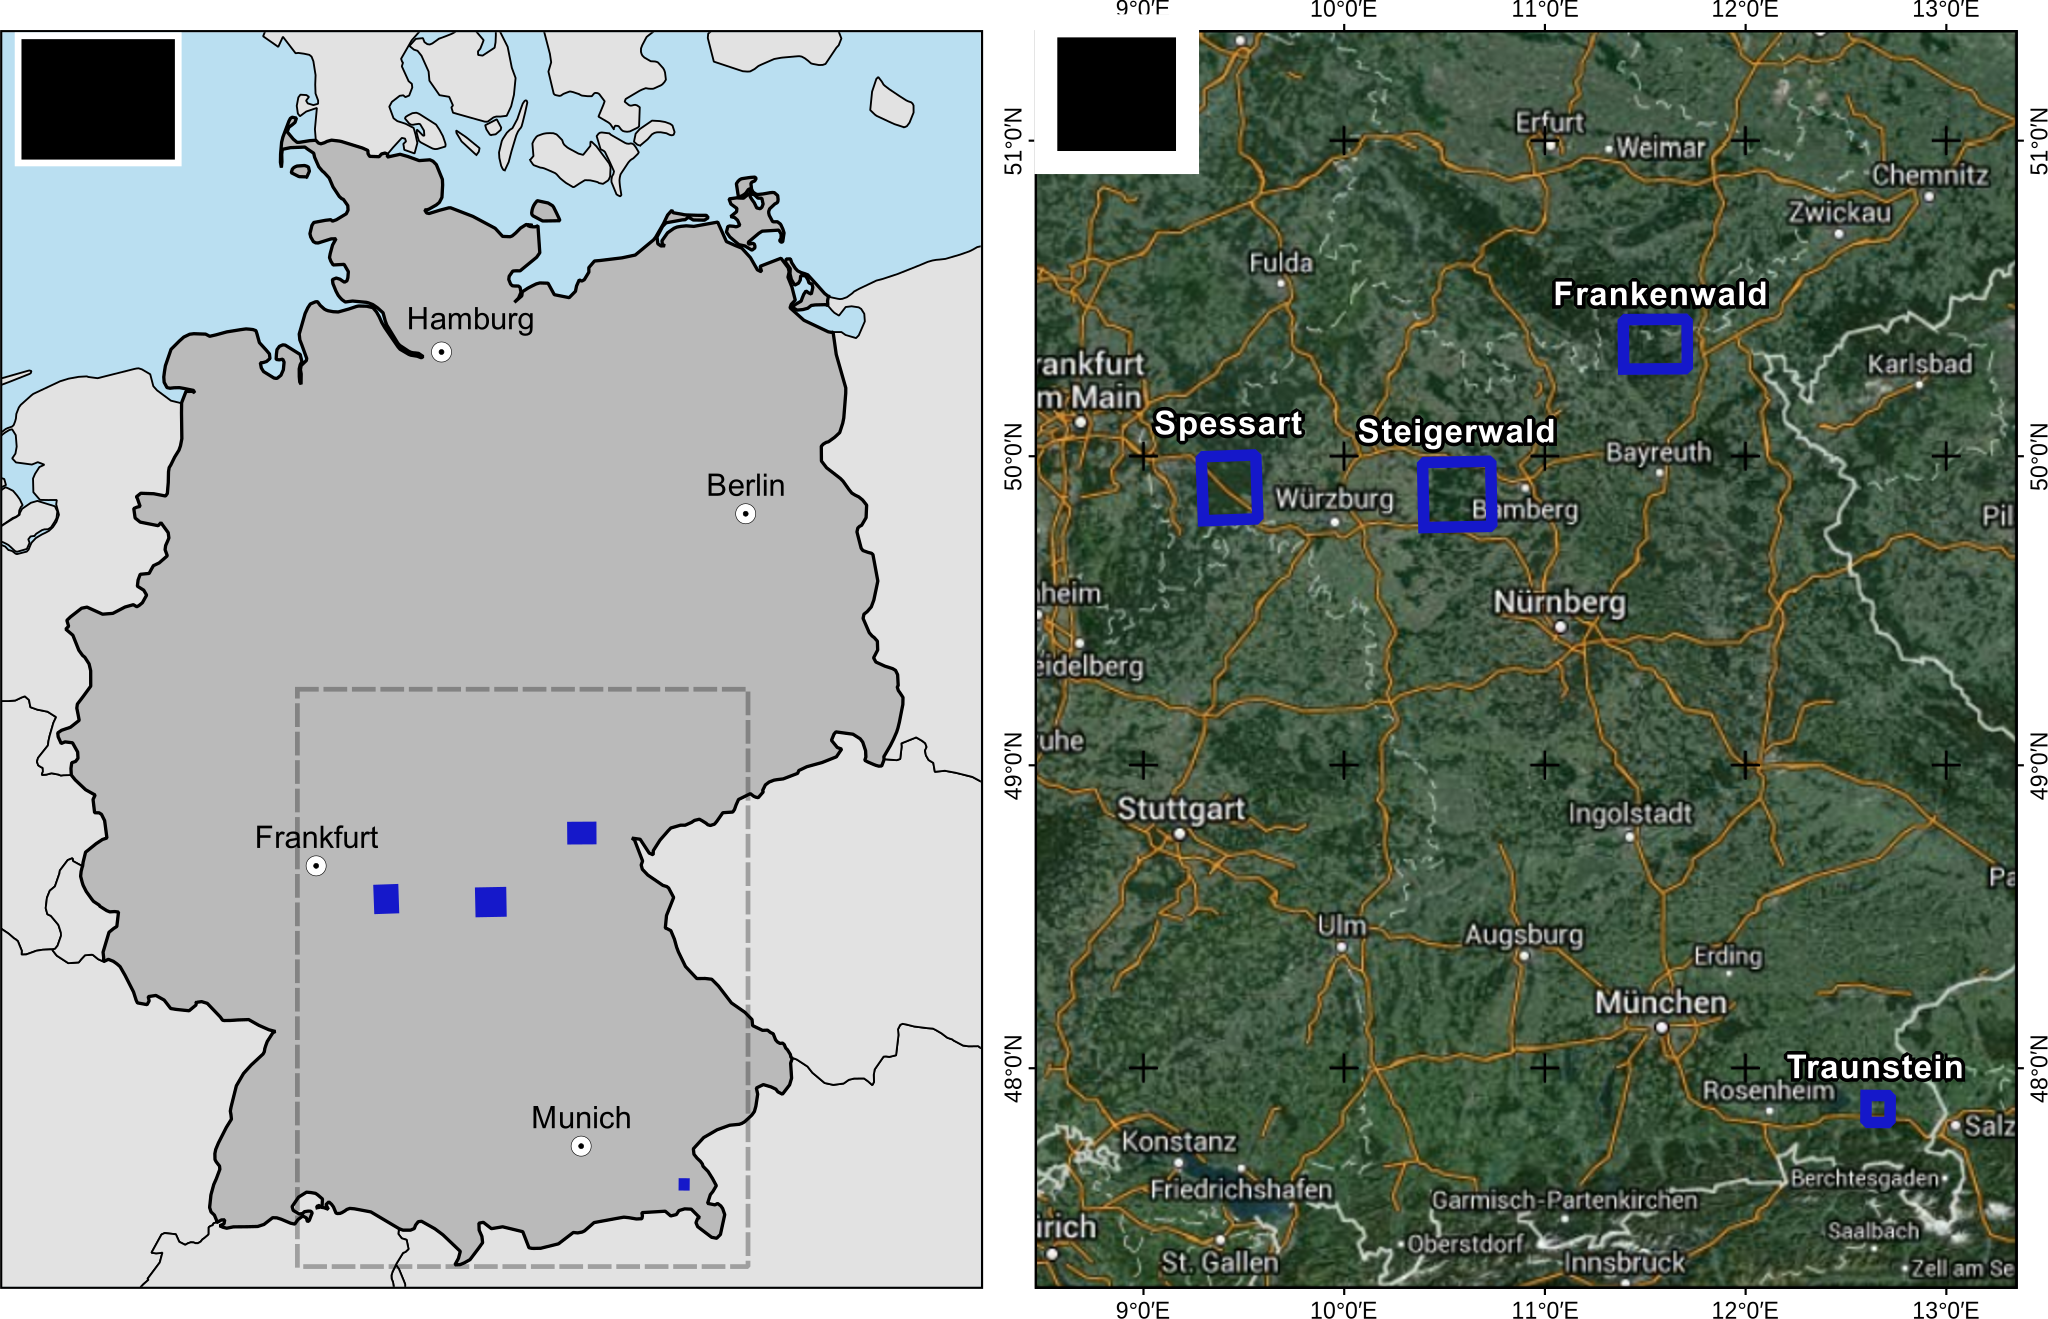
\includegraphics[width=1\textwidth]{Figures/TestSites/Bavaria/TestSites_BY_2} %scale for golden ratio 0.618
	\caption[Map of the study areas in Bavaria.]{Map of the study areas \emph{Spessart}, \emph{Steigerwald}, \emph{Frankenwald}, 
		and \emph{Traunstein} in Bavaria, Germany. (a) Location in Germany; (b) detailed locations in Bavaria 
		(Images \textcopyright Landsat, Mapdata \textcopyright
		GeoBasis-DE/BKG(\textcopyright\,2009), Google).}
	\label{fig:TestSites_BY}
\end{figure}

\begin{figure}[!h]
	\centering
	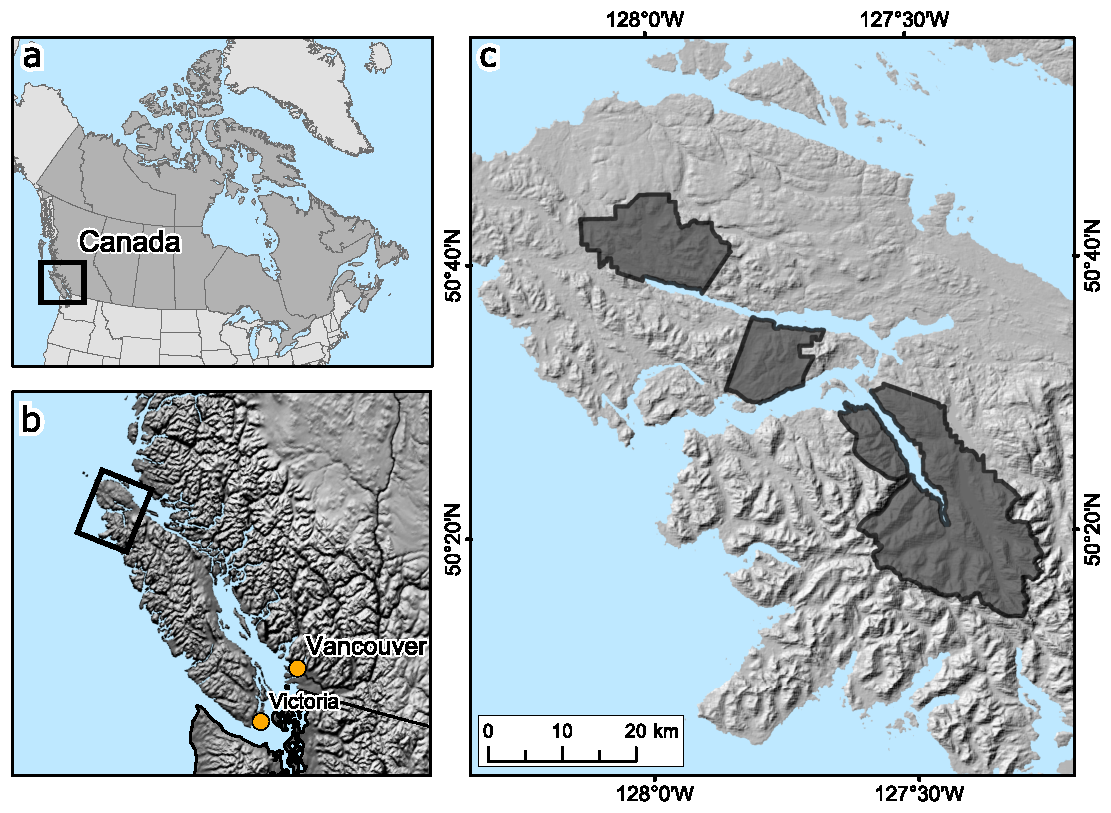
\includegraphics[width=.9\textwidth]{Figures/TestSites/NVI/wfp_BritishColumbia_testSite} %scale for golden ratio 0.618
	\caption[Map of the study area in British Columbia.]{Map of the study area \emph{Northern Vancouver Island} in 
		British Columbia, Canada. (a) Location in British Columbia, Canada;
		(b) location on \mbox{Northern} Vancouver Island; (c) boundaries of the study area units.}
	\label{fig:TestSite_NVI}
\end{figure}


\section{Field Data}\label{sec:FieldData}

\subsection{Bavarian State Forest Enterprise}\label{subsec:FieldData_BaySF}

Main parts of the test sites \emph{Spessart}\index{study area!Bavaria!Spessart}, \emph{Steigerwald}\index{study area!Bavaria!Steigerwald}, 
and \emph{Frankenwald}\index{study area!Bavaria!Frankenwald} are state-owned\index{state-owned} land, 
mostly managed forests with a great variety of stand development stages. The areas are managed by the 
\ac{BaySF}, and field data are recorded frequently according to their forest management guidelines \parencite{Neufanger.2011}.

For the respective forests, \graffito{Ground plots for terrestrial inventory measurements are permanently marked in the Bavarian state forests.} 
recurring terrestrial sample-based forest inventory systems are installed, and 
comprehensive measurements are carried out on a 10-year frequency basis.
The permanent ground plots where the data are collected are laid out in a regular grid pattern of 200\,m\;x\;200\,m.
The plot centres are permanently marked in the field, and during the inventories, each particular plot location is georeferenced 
using a GPS device. 

The forest management inventories \graffito{Tree measurements at the plots are made according to concentric sampling circles.} 
in the state forests of Bavaria make use of the sampling concept with three concentric measurement circles\index{concentric sampling circles}
at the respective ground plots. A general introduction to this concept can be found in \textcite{vanLaar.2007}. Here, the trees are recorded with 
all relevant attributes in dependency of their \acl{DBH} (\acs{DBH}; measured at 1.3\,m above ground) and their distance to the plot centre.
For the forest inventories conducted by \ac{BaySF}, the radii and \acs{DBH} thresholds for the concentric circles 
assembling a circular inventory plot typically are set as summarized in Table~\ref{tab:Radii}.

\begin{table}[htb]
	\myfloatalign
	\caption[Radii and DBH thresholds for the concentric sampling circles.]{Radii and \ac{DBH} thresholds for the concentric sampling circles
		assembling a ground plot in typical \ac{BaySF} management inventories.}
	\label{tab:Radii}
	\small
	\begin{tabularx}{.8\textwidth}{XXXX}
		\toprule
		\spacedlowsmallcaps{Circle} \linebreak \spacedlowsmallcaps{No.} & \spacedlowsmallcaps{Radius} \linebreak \footnotesize{[m]} & \spacedlowsmallcaps{Area} \linebreak \footnotesize{[m\textsuperscript{2}]} & \spacedlowsmallcaps{DBH} \linebreak \footnotesize{[cm]}  \\ 
		\midrule
		\emph{1} & 2.82 & 25 & $<$\,12  \\ 
		\emph{2} &  6.31 &  125 & 12--29.9 \\
		\emph{3}  & 12.62 &  500 & $\geq$\,30  \\ 
		\bottomrule
	\end{tabularx}
\end{table}
 
Based on the individual tree measurements, \graffito{A set of forest inventory attributes is computed based on the individual tree measurements.}
a set of forest inventory attributes\index{forest inventory attribute} is computed. 
These compiled data sets include, 
inter alia, mean tree height, basal area per hectare, and gross volume per hectare.
In the course of the research project, other attributes, \eg, stand top height, came into focus, 
and procedures were applied to compute the attributes from the individual tree measurements. 

The field data \graffito{Field data in the test sites \emph{Spessart}, \emph{Steigerwald}, and \emph{Frankenwald} were 
	acquired in 2011, 2010, and 2014.} 
for the \ac{BaySF} test sites included in this work, namely \emph{Spessart}, \emph{Steigerwald}, and \emph{Frankenwald},
were recorded in 2011, 2010, and 2014, respectively. 
For more detailed descriptions of the field data acquisitions as well as 
the derivation of forest inventory attributes, refer to the respective sections in the articles. 

\subsection{National forest inventory data}\label{subsec:NFI_data}

Field data from the German \ac{NFI}\index{national forest inventory}\index{NFI|see{national forest inventory}} were selected as reference data for 
model training in the study of \textcite{Immitzer.2016}.
Contrary to the concentric sampling circles used within the management forest inventories of \ac{BaySF},
\graffito{\ac{ACS}\index{angle-count sampling}\index{ACS|see{angle-count sampling}} is used as basic sampling principle in the German \ac{NFI}.} 
the German \ac{NFI} is based on \acf{ACS} as basic sampling principle. Here, the probability of a tree for inclusion to the measurements
is proportional to its basal area at a defined height. Each tree trunk is focused from the sample plot centre and is 
selected if the \ac{DBH} exceeds a prescribed angle width (defined by the so called basal area factor). 
For more information regarding the German \ac{NFI} and the \ac{ACS} method, refer to the corresponding section in the 
paper \parencite{Immitzer.2016} or to \textcite{Polley.2010}.

 Our study was conducted in the \emph{Steigerwald} test site, 
 and a total of 92 sample plots from the most recent \ac{NFI} were used for modelling. 
 \graffito{\ac{NFI} field data were recorded in 2011 and 2012.}The field measurements were conducted in 2011 and 2012, 
 and field-based estimates of growing stock, separately for conifers and broadleaves, 
 were made available to us. 

\subsection{Municipal Forest of Traunstein}\label{subsec:FieldData_Traunstein}

The forest area, which was chosen as test site for the study of \textcite{Stepper.2015}, is part of the municipal forest which belongs 
to the city of Traunstein\index{study area!Bavaria!Traunstein}. 
The forest stands are actively managed to support an uneven-aged mixed-species forest and comprise a 
great variety of successional stages, \ie, heterogeneous species composition, many different age classes, and multi-layered stands.

Similarly to the field sampling design described above for the \ac{BaySF} inventories (subsection~\ref{subsec:FieldData_BaySF}), 
the permanently marked field plots within the \emph{Traunstein} study area -- 228, in total -- are distributed in a regular grid pattern of 100\,m\;x\;100\,m.
At the plots, measurements are carried out using concentric sampling circles\index{concentric sampling circles}, 
based on the following radii and corresponding \ac{DBH} thresholds:
3.15\,m (\ac{DBH}\,$<$\,10\,cm), 6.31\,m (10\,$\leq$\,\ac{DBH}\,$<$\,30\,cm) and 12.62\,m (\ac{DBH}\,$\geq$\,30\,cm).

The \emph{Traunstein} forest test site \graffito{Field measurements collected in 2008 and 2013 were available 
	for the \emph{Traunstein} test site.} was selected for our experiment of assessing forest height changes 
by means of \ac{DAP}-based \acp{CHM}, as field measurements from two terrestrial inventories carried out in 2008 and 2013 were available.
Using the ground plot measurements, field-based top heights were calculated for each inventory plot, and in consequence, field-based
\acf{PAI}\index{periodic annual increment}\index{PAI|see{periodic annual increment}} could be derived as reference for our investigation. 
Details regarding the ground measurements and the subsequent calculations are given
in the respective sections of the paper \parencite{Stepper.2015}.


\subsection{Northern Vancouver Island}\index{study area!British Columbia!Northern Vancouver Island}

To select \graffito{Stratified random sampling was used to select the ground plot locations at \ac{NVI}.}
the ground plot locations in the \ac{NVI} study area, a stratified random sampling\index{stratified random sampling} design was used. 
The ground plots were allocated to five different strata, defined by species information, biogeographic data, and elevation data. 
The sample locations within the strata were selected by a systematic partition, informed by the 3d \ac{ALS}-derived feature space.

In total, 140 ground plots were established within the \ac{NVI} test site (which corresponds to a much greater area representativeness
of the individual plots compared to the ones described in subsections~\ref{subsec:FieldData_BaySF} and~\ref{subsec:FieldData_Traunstein}). 
In the field, the plot centres were established using a GPS device, and all live standing trees with \ac{DBH}\,$\geq$\,12.0\,cm were measured
within a radius of 14\,m ($615.75 m^2$). The individual tree measurements included \ac{DBH}, stem height, age and other mensurational data, 
and estimates for different forest inventory attributes, including Lorey's mean height, basal area, and gross volume, were calculated for each plot
\parencite{White.2015}.


\section{Remote Sensing Data}\label{sec:RemSensData}

This work was purposely designed to investigate digital aerial photographs\index{aerial photograph!digital aerial photograph} 
as remote sensing data for use in forest inventory and management applications. 
Thus, airphotos were the primary remotely sensed data used for analysis in this study.
Besides aerial photography, we examined stereo \acf{WV2}\index{WorldView-2} satellite data for generating 3d height measurements of forest canopies,
and the consequent use for a wall-to-wall mapping\index{wall-to-wall mapping} application of forest inventory data. 
\ac{ALS} data were used twofold: (i)~as indispensable source of information providing detailed elevation models, \ie, ground heights of the terrain; 
(ii)~as reference remote sensing data used in the \ac{ABA}\index{area-based approach} modelling of forest inventory attributes, 
\ie, to judge the achieved results when using 
\ac{DAP} derived height information.

\subsection{Digital Aerial Photographs}

The \graffito{Digital airphotos are acquired routinely by the Bavarian Administration for Surveying.} digital aerial photographs
used for the studies conducted in the Bavarian test sites (see Table~\ref{tab:TestSites}) were provided by the 
Bavarian Administration for Surveying. Currently, the aerial photographs are updated every three years in Bavaria.
General specifications for these official aerial photographs are provided in \textcite{LDBV.2015c}.

All images used in our studies were acquired during leaf-on\index{leaf-on} conditions with digital aerial frame cameras, and both 
panchromatic\index{panchromatic} (PAN) and PAN-sharpened multispectral\index{multispectral} images (blue, green, red, and near infrared) of the same 
radiometric resolution\index{resolution!radiometric} (12\,bit) were available. 
The aerial photographs were acquired such that a \ac{GSD}\index{ground sampling distance} of 0.20\,m  could be ensured for all images.   

The overlaps \graffito{The typical overlaps of the stereo images in Bavaria were 65--75\,\%  in forward and 25--40\,\% in side direction.}
of the stereo images varied between different years of data acquisition and different test sites,
but, in general, overlaps in forward\index{overlap!forward} and side\index{overlap!side} direction of 65--75\,\% and 25--40\,\% were achieved.
For details regarding the used camera type, the individual image overlaps, and the flight dates of the aerial surveys,
the reader is referred to the respective sections of the research articles.

With regard to the study conducted on \ac{NVI}, digital aerial imagery was acquired by the tree farm licensee
Western Forest Products Inc. being responsible for the management of the forests within the study area.
For complete coverage of the area, imagery was acquired during four different flights from August to October 2012.
The photographs were acquired with a minimum of 60\,\% along-track (forward) and 20\,\% across-track (side) overlap.
The airphotos were provided as 4-band (blue, green, red, near infrared) multispectral\index{multispectral} images with a 0.30\,m \ac{GSD} and 
8\,bit radiometric\index{resolution!radiometric} resolution.

\subsection{World-View 2 Data}

In the study of \textcite{Immitzer.2016} we explored the usability of high-resolution optical satellite imagery\index{optical satellite imagery} 
recorded in stereoscopic collection mode for the image-based generation of 3d height data and further application. 
Therefore, \ac{WV2} stereo satellite image data were used.
\ac{WV2} records panchromatic\index{panchromatic} images plus multispectral\index{multispectral} images 
comprising eight spectral bands (coastal, blue, green, yellow,
red, red edge, near infrared~1, near infrared~2; \cite{DigitalGlobe.2013}).
 
For the test site \emph{Steigerwald} complete coverage was achieved through two stereo-image pairs, \ie, four \ac{WV2} images,
which were recorded under leaf-on\index{leaf-on} conditions in August 2013. The spectral data were atmospherically corrected and thus, top-of-canopy
spectral reflectance was available for further analysis. 
The \ac{WV2} data were provided as panchromatic images with 0.50\,m spatial\index{resolution!spatial} resolution, 
and as 8-band multispectral images resampled to 1.0\,m pixel size.

\subsection{Airborne Laser Scanning Data}

As mentioned above, one essential benefit of \ac{ALS}\index{airborne laser scanning} 
data sets is that measurements describing the canopy structure and the ground surface 
can be acquired simultaneously. This allows for the computation of vegetation heights using inherent ground measurements.
For the \ac{DAP}-based reconstruction of vegetation height, additional bare earth information is necessary. 

The Bavarian Administration for Surveying routinely runs \ac{ALS} mapping surveys in order to achieve accurate measurements of the terrain
(however, with no distinct repeat cycle).
Based \graffito{\acp{DTM} with 1\,m ground resolution are available for the entire area of Bavaria.}
on these \ac{ALS} data, \acfp{DTM}\index{DTM|see{digital terrain model}}\index{digital terrain model} with 1\,m ground resolution
are available for the entire area of the country \parencite{LDBV.2015b}.
In the course of the research project, the \ac{ALS}-based \acp{DTM} were used for the height normalization\index{height normalization} 
of the \ac{DAP}-based surface measurements.
Canopy heights were consequently calculated as difference of the image-based surface heights and the \ac{ALS}-based terrain heights.

In the \ac{NVI} study area \ac{ALS} point clouds\index{point cloud} were acquired at the same time as the digital airphotos, \ie, in August and September 2012. 
The data had an average return point density\index{point density} of 11.6\,points$\cdot$m\textsuperscript{2}.
Based on the ground returns from that data, a \ac{DTM} with a spatial resolution of 1\,m was created. The \ac{DTM} was used to normalize the 
\ac{ALS} point cloud heights to heights above ground level. In addition, the image-based points from the \ac{NVI} study area were transformed to heights
above ground using the same \ac{ALS}-based \ac{DTM}. 


 
    

